

\tikzset{every picture/.style={line width=0.75pt}} %set default line width to 0.75pt        

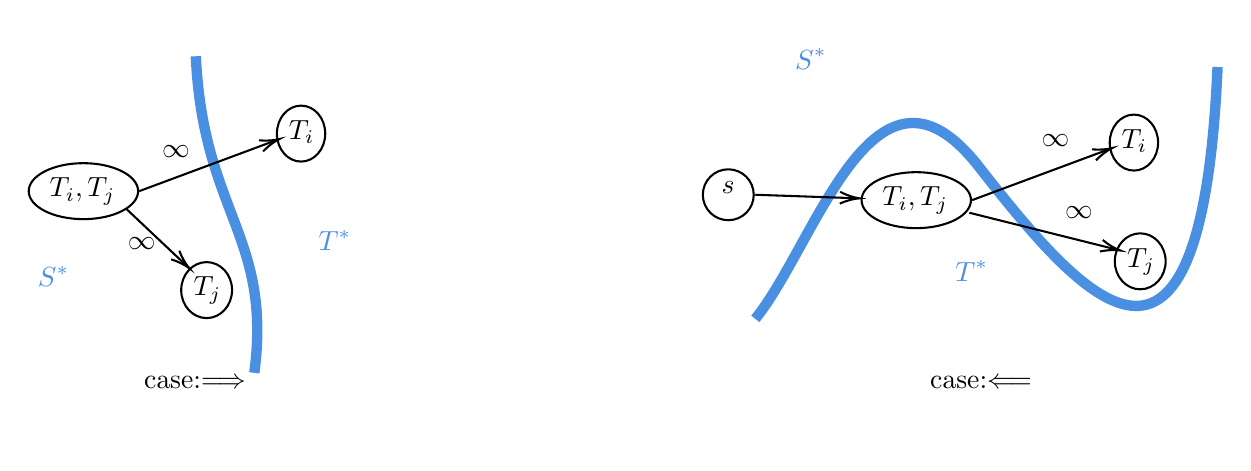
\begin{tikzpicture}[x=0.65pt,y=0.65pt,yscale=-1,xscale=1]
%uncomment if require: \path (0,459); %set diagram left start at 0, and has height of 459

%Curve Lines [id:da054999626964672865] 
\draw [color={rgb, 255:red, 74; green, 144; blue, 226 }  ,draw opacity=1 ][line width=3.75]    (166,265) .. controls (176,189) and (137.5,176) .. (133.5,89) ;
%Straight Lines [id:da2789805505394123] 
\draw    (102,164) -- (178.13,135.7) ;
\draw [shift={(180,135)}, rotate = 159.61] [color={rgb, 255:red, 0; green, 0; blue, 0 }  ][line width=0.75]    (10.93,-3.29) .. controls (6.95,-1.4) and (3.31,-0.3) .. (0,0) .. controls (3.31,0.3) and (6.95,1.4) .. (10.93,3.29)   ;
%Straight Lines [id:da48164084756462144] 
\draw    (95,174) -- (128.54,205.63) ;
\draw [shift={(130,207)}, rotate = 223.32] [color={rgb, 255:red, 0; green, 0; blue, 0 }  ][line width=0.75]    (10.93,-3.29) .. controls (6.95,-1.4) and (3.31,-0.3) .. (0,0) .. controls (3.31,0.3) and (6.95,1.4) .. (10.93,3.29)   ;
%Curve Lines [id:da16276842775686318] 
\draw [color={rgb, 255:red, 74; green, 144; blue, 226 }  ,draw opacity=1 ][line width=3.75]    (444.5,235) .. controls (478.5,193) and (510.5,76) .. (568.63,150.18) .. controls (626.75,224.35) and (692.5,301) .. (701.5,95) ;
%Straight Lines [id:da5400494970222413] 
\draw    (565,169) -- (641.13,140.7) ;
\draw [shift={(643,140)}, rotate = 159.61] [color={rgb, 255:red, 0; green, 0; blue, 0 }  ][line width=0.75]    (10.93,-3.29) .. controls (6.95,-1.4) and (3.31,-0.3) .. (0,0) .. controls (3.31,0.3) and (6.95,1.4) .. (10.93,3.29)   ;
%Straight Lines [id:da8447819866227777] 
\draw    (563.5,176) -- (645.56,196.51) ;
\draw [shift={(647.5,197)}, rotate = 194.04] [color={rgb, 255:red, 0; green, 0; blue, 0 }  ][line width=0.75]    (10.93,-3.29) .. controls (6.95,-1.4) and (3.31,-0.3) .. (0,0) .. controls (3.31,0.3) and (6.95,1.4) .. (10.93,3.29)   ;
%Straight Lines [id:da34298456292109847] 
\draw    (444.5,166) -- (500.5,167.93) ;
\draw [shift={(502.5,168)}, rotate = 181.97] [color={rgb, 255:red, 0; green, 0; blue, 0 }  ][line width=0.75]    (10.93,-3.29) .. controls (6.95,-1.4) and (3.31,-0.3) .. (0,0) .. controls (3.31,0.3) and (6.95,1.4) .. (10.93,3.29)   ;

% Text Node
\draw    (71, 164) circle [x radius= 30.41, y radius= 15.56]   ;
\draw (50.5,155) node [anchor=north west][inner sep=0.75pt]   [align=left] {$\displaystyle T_{i} ,T_{j}$};
% Text Node
\draw    (192, 132) circle [x radius= 13.44, y radius= 15.56]   ;
\draw (183.5,123) node [anchor=north west][inner sep=0.75pt]   [align=left] {$\displaystyle T_{i}$};
% Text Node
\draw (113,137) node [anchor=north west][inner sep=0.75pt]   [align=left] {$\displaystyle \infty $};
% Text Node
\draw    (139.5, 219) circle [x radius= 14.14, y radius= 15.56]   ;
\draw (130.5,210) node [anchor=north west][inner sep=0.75pt]   [align=left] {$\displaystyle T_{j}$};
% Text Node
\draw (94,188) node [anchor=north west][inner sep=0.75pt]   [align=left] {$\displaystyle \infty $};
% Text Node
\draw (200,184) node [anchor=north west][inner sep=0.75pt]  [color={rgb, 255:red, 74; green, 144; blue, 226 }  ,opacity=1 ] [align=left] {$\displaystyle \textcolor[rgb]{0.29,0.56,0.89}{T}\textcolor[rgb]{0.29,0.56,0.89}{^{*}}$};
% Text Node
\draw (44,204) node [anchor=north west][inner sep=0.75pt]  [color={rgb, 255:red, 74; green, 144; blue, 226 }  ,opacity=1 ] [align=left] {$\displaystyle \textcolor[rgb]{0.29,0.56,0.89}{S}\textcolor[rgb]{0.29,0.56,0.89}{^{*}}$};
% Text Node
\draw    (534, 169) circle [x radius= 30.41, y radius= 15.56]   ;
\draw (513.5,160) node [anchor=north west][inner sep=0.75pt]   [align=left] {$\displaystyle T_{i} ,T_{j}$};
% Text Node
\draw    (655, 137) circle [x radius= 13.44, y radius= 15.56]   ;
\draw (646.5,128) node [anchor=north west][inner sep=0.75pt]   [align=left] {$\displaystyle T_{i}$};
% Text Node
\draw (602,131) node [anchor=north west][inner sep=0.75pt]   [align=left] {$\displaystyle \infty $};
% Text Node
\draw    (658.5, 203) circle [x radius= 14.14, y radius= 15.56]   ;
\draw (649.5,194) node [anchor=north west][inner sep=0.75pt]   [align=left] {$\displaystyle T_{j}$};
% Text Node
\draw (615,171) node [anchor=north west][inner sep=0.75pt]   [align=left] {$\displaystyle \infty $};
% Text Node
\draw (554,201) node [anchor=north west][inner sep=0.75pt]  [color={rgb, 255:red, 74; green, 144; blue, 226 }  ,opacity=1 ] [align=left] {$\displaystyle \textcolor[rgb]{0.29,0.56,0.89}{T}\textcolor[rgb]{0.29,0.56,0.89}{^{*}}$};
% Text Node
\draw (465,83) node [anchor=north west][inner sep=0.75pt]  [color={rgb, 255:red, 74; green, 144; blue, 226 }  ,opacity=1 ] [align=left] {$\displaystyle \textcolor[rgb]{0.29,0.56,0.89}{S}\textcolor[rgb]{0.29,0.56,0.89}{^{*}}$};
% Text Node
\draw    (429.5, 166) circle [x radius= 14.15, y radius= 14.15]   ;
\draw (424,157) node [anchor=north west][inner sep=0.75pt]   [align=left] {$\displaystyle s$};
% Text Node
\draw (103,265.5) node [anchor=north west][inner sep=0.75pt]   [align=left] {case:$\displaystyle \Longrightarrow $};
% Text Node
\draw (540,265.5) node [anchor=north west][inner sep=0.75pt]   [align=left] {case:$\displaystyle \Longleftarrow $};


\end{tikzpicture}

